% Figure — Modèle de Shannon et Weaver (TS227, chapitre 1).
% D'après le support [poly, p. 11 à 14], redessinée.
% Rendu SVG :
%   latex -output-directory=<dossier temporaire> 01-shannon-weaver.tex
%   dvisvgm --no-fonts --exact-bbox -o 01-shannon-weaver.svg <dossier temporaire>/01-shannon-weaver.dvi
\documentclass[tikz,border=4pt]{standalone}
\usepackage[T1]{fontenc}
\usepackage[utf8]{inputenc}
\usepackage{sansmath}
\renewcommand{\familydefault}{\sfdefault}
\usetikzlibrary{positioning,arrows.meta}
\begin{document}
\sansmath
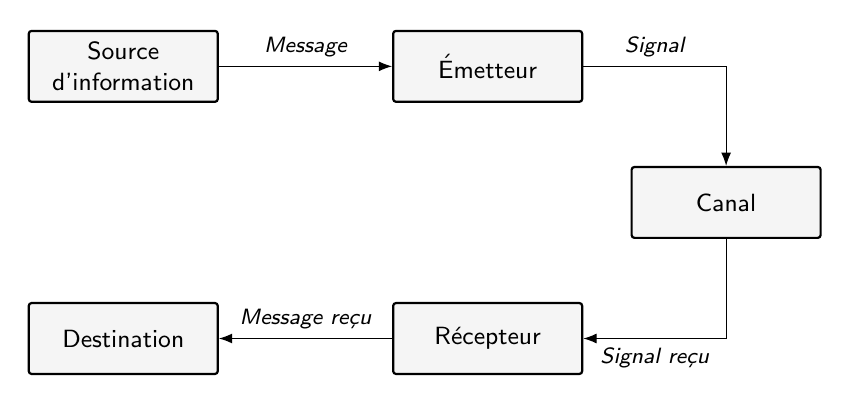
\begin{tikzpicture}[
    >=Latex, font=\small,
    bloc/.style={draw, thick, rounded corners=1pt, minimum height=9mm, minimum width=24mm, align=center, fill=black!4},
    sig/.style={font=\footnotesize\itshape},
  ]
  \node[bloc] (src) {Source\\d'information};
  \node[bloc, right=22mm of src] (em) {Émetteur};
  \node[bloc, below right=8mm and 6mm of em] (canal) {Canal};
  \node[bloc, below left=8mm and 6mm of canal] (rec) {Récepteur};
  \node[bloc, left=22mm of rec] (dst) {Destination};
  \draw[->] (src) -- node[above, sig] {Message} (em);
  \draw[->] (em.east) -| node[above, sig, pos=0.25] {Signal} (canal.north);
  \draw[->] (canal.south) |- node[below, sig, pos=0.75] {Signal reçu} (rec.east);
  \draw[->] (rec) -- node[above, sig] {Message reçu} (dst);
\end{tikzpicture}
\end{document}
